%\documentclass[12pt,serif]{beamer}
%\documentclass[tikz,12pt,svgnames]{beamer}
\documentclass[table,handout,tikz,12pt,svgnames]{beamer}
\usepackage{CM-preamble}
\subtitle{\Huge Recursivité}
\date{11 février 2016}

%README TODO STUFF
%README This presentation is not as well made as previous ones. For example, pseudo code is not underlined and some things are not well aligned.

\begin{document}

\begin{frame}
	\titlepage
\end{frame}

\begin{frame}[fragile=singleslide]
	\frametitle{La récursivité: Liste chaînée}
%\vspace{-0.7cm}
\begin{center} \noindent\makebox[\linewidth]{
\begin{tikzpicture}
%%\foreach \index/\list in {1/{a,b,null}, 2/{c,null}, 3/{d,null}} {
\foreach \index/\list in {1/{$a_0$,$a_2$,$a_3$,$a_4$}} {
	\node[array element] (aux) at (0,-\index) {L};
    \LinkedList{\list}
}
\node at (2.5,-2) {\texttt{<elt>}};
\draw[dash pattern=on 6pt off 3pt, line width = 0.7mm] (3.5,-0.2) -- (3.5,-2.4) ;
\node at (6.5,-2) {\texttt{<liste>}};
\draw[dash pattern=on 6pt off 3pt, line width = 0.7mm] (9.65,-0.2) -- (9.65,-2.4) ;
\node at (10.2,-2) {\texttt{$\emptyset$}};

%\draw[<->] ([shift={(0,-1)}]-1,-1) --  ([shift={(-2,-2)}]4.2,-1);
%\draw[<->] ([shift={(0.5,0.5)}]4.4,-1) --node[below] {Zone d'extension contigue} ([shift={(0.5,0.5)}]9.6,-1);

\end{tikzpicture}
}
\end{center}
	\vspace{-0.9cm}
		\begin{block}{} %Gestion dynamique de la mémoire}
			\begin{itemize}
			\item Structure de données récursive :\\
			\texttt{<liste> ::= <elt> <liste> | $\emptyset$ }
			\end{itemize}
		\end{block}
	  \begin{columns}[c]
  		\hspace{-0.5cm}
	  	\begin{column}{0.7\textwidth}
		\begin{block}{Déclaration} %Gestion dynamique de la mémoire}
			\begin{minted}[mathescape=true,escapeinside=||,tabsize=4,fontsize=\footnotesize,]{c}
	type Liste = pointeur de Cellule
	type Cellule = structure 
		 valeur : <T>
		 suivant : Liste
	fin
			\end{minted}
		\end{block}
		\end{column}
%		\setlength{\columnseprule}{0.4pt}
		\hspace{-1.3cm}
		\vrule{}
		\hspace{0.3cm}	
		\begin{column}{0.38\textwidth}
		Récursivité croisée	(ou indirecte)
	    \end{column}
	\end{columns}
\end{frame}


\begin{frame}[fragile=singleslide]
	\frametitle{La récursivité}
		\vspace{-0.8cm}
		\begin{block}{} %Gestion dynamique de la mémoire}
			\begin{itemize}
				\item Une entité (SD, algorithme) est récursive si elle se définit à partir d'elle 
				même		
				\item Algorithmes récursifs (exemple : factorielle, fibonacci)
				%\begin{itemize}
				\vspace{0.3cm}
				\begin{block}{Exemple d'algo récursive: Factorielle}
					\item Analyse récurrente
					\begin{itemize}
						\item $ n! = n * (n-1)!$
						\item $ 0! = 1 $								
					\end{itemize}
				\vspace{0.5cm}
				\hspace{-2cm}
				\item Écriture fonctionnelle
				\begin{columns}[b]
				  	\hspace{-0.3cm}
				  	\begin{column}{0.55\textwidth}
						\begin{itemize}
							\item \texttt{fact(n) = n * fact(n-1)}
						\end{itemize}
					\end{column}
			%		\setlength{\columnseprule}{0.4pt}
					\hspace{-0.3cm}
					\vrule{}
					\hspace{0cm}	
					\begin{column}{0.45\textwidth}
						\begin{itemize}
							\item Cas générale, récursif
						\end{itemize}
				    \end{column}
				\end{columns}
				\begin{columns}[c]
				  	\hspace{-0.3cm}
				  	\begin{column}{0.55\textwidth}
						\begin{itemize}
							\item \texttt{fact(0) = 1}
						\end{itemize}
					\end{column}
			%		\setlength{\columnseprule}{0.4pt}
					\hspace{-0.33cm}
					\vrule{}
					\hspace{0cm}	
%					\vspace{5cm}
					\begin{column}{0.45\textwidth}
						\begin{itemize}
							\item Cas primitif, terminal
						\end{itemize}
				    \end{column}
				\end{columns}
				\end{block}					
				%\end{itemize}
			\end{itemize}
		\end{block}
\end{frame}

%TODO UNDERLINES
\begin{frame}[fragile=singleslide]
	\frametitle{Factorielle}
%		\vspace{-0.8cm}
%				\begin{columns}[T]
%				  	\hspace{-0.3cm}
%				  	\begin{column}{0.5\textwidth}
%				  	\begin{block}{}
\vspace{-0.15cm}
						\begin{minted}[mathescape=true,escapeinside=||,tabsize=3,		fontsize=\footnotesize]{text}
Action Dichotomie(L,X,G,D,pos,existe)
	D : L : liste contiguë d'entiers
	X, G, D : entier
	R : pos: entier ; existe : booléen
	L : M : entier
	Si G>D Alors
		existe |$\leftarrow$| faux
	Sinon
		M |$\leftarrow$| (G + D) / 2
		Si X = L.espace[M] Alors
			existe |$\leftarrow$| vrai
			pos |$\leftarrow$| M
		Sinon
			Si X < L.espace[M] Alors
				dichotomie(L,X,G,M-1,pos,existe)
			Sinon
				dichotomie(L,X,M+1,D,pos,existe)
			Fsi
		Fsi
	Fsi
Faction
						\end{minted}		
%					\end{block}			
%					\end{column}
%			%		\setlength{\columnseprule}{0.4pt}
%%					\hspace{-0.25cm}
%					\vrule{}
%%					\hspace{0cm}	
%%					\vspace{5cm}
%				  	\begin{column}{0.55\textwidth}
%				  	\begin{block}{}
%						\begin{minted}[mathescape=true,escapeinside=||,tabsize=3,		fontsize=\footnotesize]{c}
%						\end{minted}					
%					\end{block}	
%					\end{column}
%				\end{columns}
\end{frame}

\begin{frame}[fragile=singleslide]
	\frametitle{Exemple d'exécution d'une factorielle}
	{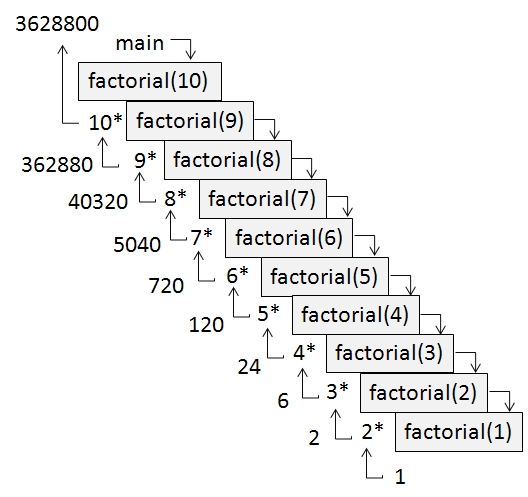
\includegraphics[scale=0.50]{../common-images/RecursiveFactorial.jpg}}
\end{frame}

\begin{frame}[fragile=singleslide]
	\frametitle{Conception récursive d'algorithmes}
	\begin{block}{3 parties} %Gestion dynamique de la mémoire}
		\begin{itemize}
			\item \textbf{Cas généraux récursifs:} \\ Résolution du problème par lui même
			\item \textbf{Cas terminaux non récursifs:} \\ Résolution immédiate du problème)
			\item \textbf{Conditions de terminaison} 
		\end{itemize}
	\end{block}
\end{frame}

\begin{frame}[fragile=singleslide]
	\frametitle{Exemple : Série de Fibonacci}
	\begin{minted}[mathescape=true,escapeinside=||,tabsize=4]{c}
	\end{minted}
\end{frame}




\begin{frame}[fragile=singleslide]
	\frametitle{Recherche dichotomique dans une liste contiguë: trouver l'élément \texttt{x}}
	\begin{block}{3 parties} %Gestion dynamique de la mémoire}
		\begin{itemize}
			\item Dichotomie sur \texttt{L.espace}
			\item TODO: IMAGE TABLEAU
			\item
			\item Cas général: \texttt{X $\ne$ L.espace[M]}  $\Rightarrow$ dichotomie à gauche ou à droite
			\item Cas terminal : \texttt{X = L.espace[M]}
			\item Condition de terminaison : \texttt{G > D} (non trouvé)	
		\end{itemize}
	\end{block}
\end{frame}


\begin{frame}[fragile=singleslide]
	\frametitle{Recherche dichotomique: Liste contiguë}
%		\vspace{-0.8cm}
				\begin{columns}[T]
				  	\hspace{-0.3cm}
				  	\begin{column}{0.5\textwidth}
				  	\begin{block}{Algorithme}
						\begin{minted}[mathescape=true,escapeinside=||,tabsize=3]{c}
Action Dichotomie(L,X,G,D,pos,existe)
D : L : liste contiguë d'entiers
X, G, D : entier
R : pos: entier ; existe : booléen
L : M : entier
Si G>D Alors
existe faux
Sinon
M  (G + D) / 2
Si X = L.espace[M] Alors
						\end{minted}		
					\end{block}			
					\end{column}
			%		\setlength{\columnseprule}{0.4pt}
%					\hspace{-0.25cm}
					\vrule{}
%					\hspace{0cm}	
%					\vspace{5cm}
				  	\begin{column}{0.55\textwidth}
				  	\begin{block}{Fonction}
						\begin{minted}[mathescape=true,escapeinside=||,tabsize=3]{c}
int fact (int n) {
	if (n==0)
		return 1;
	else
		return(n * fact(n-1));
}
						\end{minted}					
					\end{block}	
					\end{column}
				\end{columns}
\end{frame}





\begin{frame}[fragile=singleslide]
\end{frame}





% % % % % % % % % % % % % % % % % % % % % % % % % % %
% END
% % % % % % % % % % % % % % % % % % % % % % % % % % %



\begin{frame}[fragile=singleslide]
	\frametitle{Erreur d'allocation }
\begin{minted}[mathescape=true,escapeinside=||,tabsize=4]{c}
/* À ne pas faire */	

int * allouer_entier() {
	int var_static ; //allocated on the stack
	printf("var_static address is : %p\n",
							  &var_static);
	return &var_static ;
}			
\end{minted}
\end{frame}

\begin{frame}[fragile=singleslide]
	\frametitle{Allocation dynamique --- malloc}
		\begin{block}{Fonction \texttt{malloc}} %Gestion dynamique de la mémoire}
			\begin{itemize}
				\item \texttt{void * malloc (int taille);}
				\begin{itemize}
					\item Alloue dynamiquement dans le tas un espace de \texttt{taille} octets
					\item Résultat : \textit{pointeur non typé} vers la zone allouée
					\item Pointeur peut être converti automatiquement vers le type désiré (conversion implicite)
					\item Besoin de \texttt{\#include<stdlib.h>}
				\end{itemize}
			\end{itemize}
		\end{block}
\end{frame}

\begin{frame}[fragile=singleslide]
	\frametitle{Allocation dynamique --- Exemples}
		\begin{block}{Allocation dynamique d'un entier} %Gestion dynamique de la mémoire}
			\begin{minted}[mathescape=true,escapeinside=||,tabsize=4]{c}			
	int *pt;
	pt = (int *) malloc(sizeof(int));
	*pt = 42; //utilisation
			\end{minted}
		\end{block}
		\begin{block}{Allocation dynamique d'un tableau d'entiers}
		\end{block}
\end{frame}

%\begin{frame}[fragile=singleslide]
%	\frametitle{Allocation dynamique --- Structures}
%		\begin{block}{} %Gestion dynamique de la mémoire}
%			\begin{minted}[mathescape=true,escapeinside=||,tabsize=4]{c}	
%typedef struct {
%	int j,m,a;
%} Date;
%
%Date *pDate= (Date *) malloc(sizeof(Date));
%
%/*ex. utilisation :*/
%scanf("%d%d%d"&(pDate->j),
%				   &(pDate->m),
%				   &(pDate->a));
%			\end{minted}
%		\end{block}
%\end{frame}

\begin{frame}[fragile=singleslide]
	\frametitle{Allocation dynamique --- Structures}
		\begin{block}{} %Gestion dynamique de la mémoire}
		\vspace{-0.5cm}
		\inputminted[
%		frame=lines,
%		framesep=2.5mm,
		baselinestretch=0.7,
		fontsize=\footnotesize,
		linenos,
		tabsize=4,
%		bgcolor=light-gray
		]
		{c}{../codes/struct_declare.c}
		\end{block}
\end{frame}

%\begin{frame}[fragile=singleslide]
%	\frametitle{Allocation dynamique --- Structures}
%		\begin{block}{Tableau de structures} %Gestion dynamique de la mémoire}
%			\begin{minted}[mathescape=true,escapeinside=||,tabsize=2]{c}
%	int n; Date *pt; /*variables*/
%	scanf("%d", &n); /*taille du tableau*/
%	
%	/*pt = (Date *) malloc( n * sizeof(Date));*/
%	pt = malloc( n * sizeof *pt);
%	
%	/*utilisation:*/
%	scanf("%d%d%d", &(pt[0].j), &pt[0].m, &pt[0].a);
%
%	printf("Date %d/%d/%d\n", pt[0].j,
%													  pt[0].m,
%													  pt[0].a);
%	free(pt); pt = NULL;
%			\end{minted}
%		\end{block}
%\end{frame}

\begin{frame}[fragile=singleslide]
	\frametitle{Allocation dynamique --- Structures}
		\begin{block}{Tableau de structures} %Gestion dynamique de la mémoire}
%		\vspace{-0.5cm}
		\inputminted[
%		frame=lines,
%		framesep=2.5mm,
%		baselinestretch=0.8,
		fontsize=\small,
%		linenos,
		tabsize=2,
		firstline=16,lastline=27
%		bgcolor=light-gray
		]
		{c}{../codes/struct_declare_array.c}
		\end{block}
\end{frame}

\begin{frame}[fragile=singleslide]
	\frametitle{Allocation dynamique --- Liste contiguë}
%		\begin{block}{}
%		\vspace{-0.5cm}
		\inputminted[
%		frame=lines,
%		framesep=2.5mm,
%		baselinestretch=0.8,
		fontsize=\small,
%		linenos,
		tabsize=2,
		firstline=14,lastline=28
%		bgcolor=light-gray
		]
		{c}{../codes/alloc_listes_double_pointer.c}
%		\end{block}
\end{frame}

\begin{frame}[fragile=singleslide]
	\frametitle{Allocation dynamique --- Liste contiguë}
%		\begin{block}{}
%		\vspace{-0.5cm}
		\inputminted[
%		frame=lines,
%		framesep=2.5mm,
%		baselinestretch=0.8,
		fontsize=\small,
%		linenos,
		tabsize=2,
		firstline=44,lastline=58
%		bgcolor=light-gray
		]
		{c}{../codes/alloc_listes_double_pointer.c}
%		\end{block}
\end{frame}

\begin{frame}[fragile=singleslide]
	\frametitle{Fonction \texttt{free}}
	\begin{block}{} %Gestion dynamique de la mémoire}
		\begin{itemize}
			\item \texttt{void free(void *ptr);}
			\begin{itemize}
				\item libère l'espace mémoire pointé par \texttt{ptr} (précédemment 
				alloué)
			\end{itemize}
		\end{itemize}
	\end{block}
	\begin{block}{}
		\begin{itemize}
			\item Exemple d'utilisation:\\\textit{Suppression du dernier élément de la liste}
		\end{itemize}
		\begin{minted}[mathescape=true,escapeinside=||,tabsize=4]{c}			
		free(l.espace[l.dernier]);
		l.dernier -= 1;
		\end{minted}
	\end{block}
\end{frame}

\begin{frame}[fragile=singleslide]
	\frametitle{Listes chaînées --- Implantation en C}
%		\begin{block}{}
%		\vspace{-0.5cm}
		\inputminted[
%		frame=lines,
%		framesep=2.5mm,
%		baselinestretch=0.8,
		fontsize=\small,
%		linenos,
		tabsize=2,
		firstline=4,lastline=10
%		bgcolor=light-gray
		]
		{c}{../codes/alloc_implantation.c}
%		\end{block}
	\vspace{-0.9cm} \begin{center} \noindent\makebox[\linewidth]{\line(2,0){500}} \end{center}  \vspace{-0.7cm}
		\inputminted[
%		frame=lines,
%		framesep=2.5mm,
%		baselinestretch=0.8,
		fontsize=\small,
%		linenos,
		tabsize=2,
		firstline=13,lastline=14
		]
		{c}{../codes/alloc_implantation.c}
	\vspace{-0.9cm} \begin{center} \noindent\makebox[\linewidth]{\line(2,0){500}} \end{center}  \vspace{-0.7cm}
		\inputminted[
%		frame=lines,
%		framesep=2.5mm,
%		baselinestretch=0.8,
		fontsize=\small,
%		linenos,
		tabsize=2,
		firstline=16,lastline=20
		]
		{c}{../codes/alloc_implantation.c}
\end{frame}

\begin{frame}[fragile=singleslide]
	\frametitle{Listes chaînées --- Implantation en C}
%		\begin{block}{}
%		\vspace{-0.5cm}
		\inputminted[
%		frame=lines,
%		framesep=2.5mm,
%		baselinestretch=0.8,
		fontsize=\small,
%		linenos,
		tabsize=2,
		firstline=29,lastline=32
%		bgcolor=light-gray
		]
		{c}{../codes/alloc_implantation.c}
%		\end{block}
		\begin{center} \noindent\makebox[\linewidth]{\line(2,0){500}} \end{center} 
		\inputminted[
%		frame=lines,
%		framesep=2.5mm,
%		baselinestretch=0.8,
		fontsize=\small,
%		linenos,
		tabsize=2,
		firstline=35,lastline=39
		]
		{c}{../codes/alloc_implantation.c}
\end{frame}

\begin{frame}[fragile=singleslide]
	\frametitle{Listes chaînées --- Recherche d'un élément}
		\inputminted[
%		frame=lines,
%		framesep=2.5mm,
%		baselinestretch=0.8,
%		fontsize=\small,
%		linenos,
		tabsize=4,
		firstline=44,lastline=54
		]
		{c}{../codes/alloc_implantation.c}
\end{frame}

\begin{frame}[fragile=singleslide]
	\frametitle{Listes chaînées --- Exemple: ajout en tête}
		\inputminted[
%		frame=lines,
%		framesep=2.5mm,
%		baselinestretch=0.8,
%		fontsize=\small,
%		linenos,
		tabsize=4,
		firstline=57,lastline=73
		]
		{c}{../codes/alloc_implantation.c}
\end{frame}
%
%\begin{frame}
%\huge \center END
%\end{frame}


% % % % % % % % % % % % % % % % % % % % % % % % % % %
% END
% % % % % % % % % % % % % % % % % % % % % % % % % % %
\end{document}


% % % % % % % % % % % % % % % % % % % % % % % % % % %
% END
% % % % % % % % % % % % % % % % % % % % % % % % % % %

	\vspace{-0.9cm} \begin{center} \noindent\makebox[\linewidth]{\line(2,0){500}} \end{center}  \vspace{-0.7cm}
	\vspace{-0.9cm} \begin{center} \noindent\makebox[\linewidth]{\rule{\paperwidth}{1.5pt}}  \end{center}  \vspace{-0.7cm}	